% Valentino Vranic
% Metody inzinierskej prace 2012/13

\documentclass{beamer}

%\usetheme{Warsaw}
%\usetheme{Antibes}
\usetheme{JuanLesPins}
%\usetheme{Goettingen}

\usecolortheme{seahorse}
%\usecolortheme{dolphin}
%\usecolortheme{rose}
% http://deic.uab.es/~iblanes/beamer_gallery/index_by_color.html
%\usecolortheme{beaver}

%\useoutertheme[]{sidebar}

\setbeamercovered{transparent}

\usepackage[slovak]{babel}
\usepackage[T1]{fontenc}
\usepackage[utf8]{inputenc}
\usepackage{url}

\usepackage{listings}

\lstset{language=C++,basicstyle=\fontsize{8}{9.6}\selectfont,showstringspaces=false,columns=fullflexible,identifierstyle=\ttfamily,keywordstyle=\bfseries,showstringspaces=false,columns=fullflexible}
%\lstset{language=C,basicstyle=\fontsize{10.5}{12.6}\selectfont,identifierstyle=\ttfamily,keywordstyle=\bfseries,showstringspaces=false,columns=fixed}

\def\BibTeX{\textsc{Bib}\kern-.08em\TeX} 

\newcommand{\footcite}[1]{\footnote{\tiny #1}}
\newcommand{\umlet}{.5}
\newcommand{\emp}[1]{\textit{\alert{#1}}}
\newcommand{\kw}[1]{\mbox{\textbf{#1}}}
\newcommand{\id}[1]{\texttt{#1}}
\newcommand{\stl}{\guillemotleft}
\newcommand{\str}{\guillemotright}

\newcommand{\lsti}{\lstinline[basicstyle=\fontsize{10.5}{12.1}\selectfont]}

\newcommand{\ssection}[1]{
	\section{#1}
	\begin{frame}[fragile=singleslide]\frametitle{}
	\Huge #1
	\end{frame}
}

\newcommand{\ssectionn}[1]{
	\section*{#1}
	\begin{frame}[fragile=singleslide]\frametitle{}
	\Huge #1
	\end{frame}
}

\newenvironment{program}{\begin{beamercolorbox}[rounded=true,shadow=true]{block body}\vspace{-4mm}}{\vspace{-2mm}\end{beamercolorbox}}

\setbeamercolor{fvystup}{fg=white,bg=black}
\newenvironment{vystup}{\begin{beamercolorbox}[rounded=true,shadow=true]{fvystup}}{\end{beamercolorbox}}

\newenvironment{poznamka}{\begin{beamercolorbox}[rounded=true,shadow=false]{block body}}{\end{beamercolorbox}}

\setbeamertemplate{footline}[page number]
{
%\insertpagenumber
%\begin{beamercolorbox}{section in head/foot}
%\vskip2pt\insertnavigation{\paperwidth}\vskip2pt
%\end{beamercolorbox}%
}



\author{Ákos Lévárdy}
%\url{www.fiit.stuba.sk/~vranic}, \url{vranic@fiit.stuba.sk}}
%{\tiny \url{www.fiit.stuba.sk/~vranic}, \url{vranic@fiit.stuba.sk}}
\institute{
	Ústav informatiky, informačných systémov a softvérového inžinierstva\\
	Fakulta informatiky a informačných technológií\\
	Slovenská technická univerzita v Bratislave}

\subtitle{\vspace{3mm} Metódy inžinierskej práce 2022/2023}

\title{Závislosť študentov na hrách}

\date{\footnotesize 5. november 2020}

\begin{document}

\begin{frame}[fragile=singleslide]
\titlepage
\end{frame}

\begin{frame}[fragile=singleslide]\frametitle{Úvod}
Motivácia\\
Masívne multiplayerové online hry na hranie rolí MMORPG, sú jednou z najrýchlejšie rastúcich foriem závislosti na internete, najmä medzi deťmi a dospievajúcimi. Podobne ako závislosť od alkoholu alebo drog, aj hráči vykazujú niekoľko klasických príznakov závislosti.\\
Nadmerné hranie môže viesť ku zdravotným problémom, ale ak existuje problém, tak existuje k nemu aj riešenie.\\
Záverečné poznámky.
\end{frame}

\begin{frame}[fragile=singleslide]\frametitle{Závislosť}
\tableofcontents
Návykovosť je spôsobená tým, ako sa hry aj napríklad sociálne siete vytvárajú. 
Samotné hry nemajú dostatočnú silu vyvolať závislosť, pokiaľ daný hráč nemá určité vlastnosti. 
Závislosť znamená hrať hry každodenne viac hodín a väčšinou nie kvôli svojej vôle, ale kvôli pocitu, že potrebujem hrať a nebyť schopný dobrovoľne prestať. Závislosť ovláda správanie sa človeka. Otázkou je prečo práve hráme hry? Najprv mnoho ľudí začne hrať totiž je to dočasný únik od reality. 
\end{frame}

\begin{frame}[fragile=singleslide]\frametitle{Odrážky}
\begin{itemize}
\item Odrážky na prvej úrovni
\item Viac
	\begin{itemize}
	\item Druhá úroveň
	\item Viac
	\end{itemize}
\item Prvá úroveň
\end{itemize}
\end{frame}

\begin{frame}[fragile=singleslide]\frametitle{Odrážky}
\begin{itemize}
\item Odrážky na prvej úrovni
\item Viac
	\begin{itemize}
	\item Druhá úroveň
	\item Viac
	\end{itemize}
\item Prvá úroveň
\end{itemize}
\end{frame}


\begin{frame}[fragile=singleslide]\frametitle{Slajd len s obrázkom}
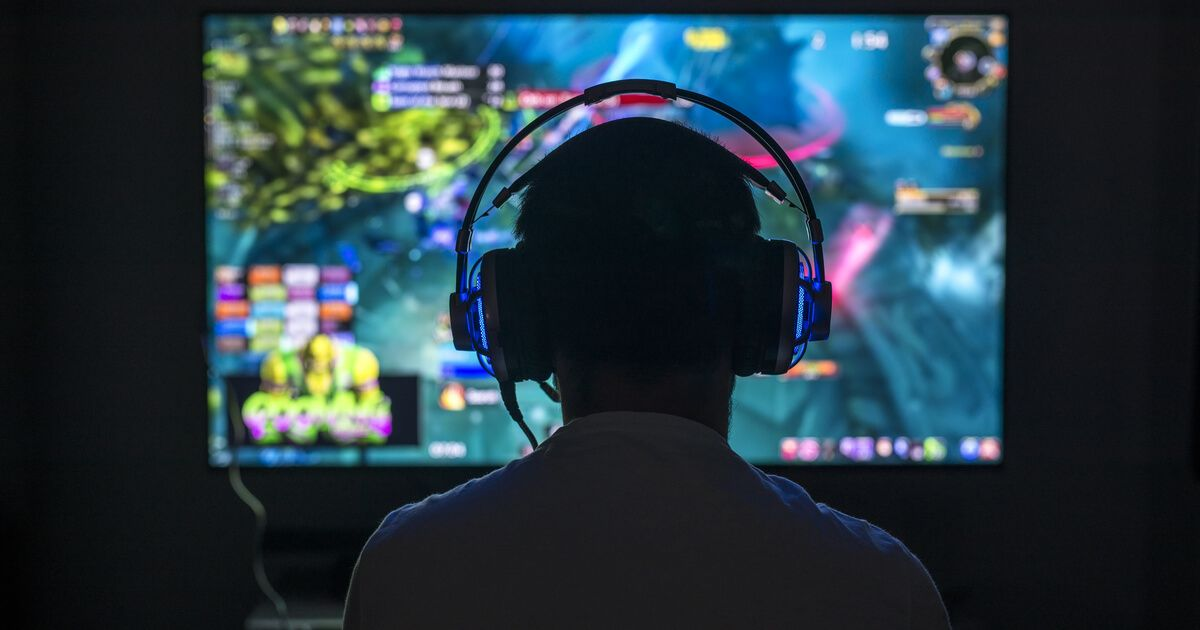
\includegraphics[scale=.35]{Video-game-addiction-(1)-guide-detail.jpg}
% pridajte vlastný obrázok a zrušte znák % pred príkazom \includegraphics vo formáte PDF prípadne PNG alebo JPG
% scale určuje veľkosť obrázku
\end{frame}

\end{document}
